\documentclass[11pt, oneside]{article}   	% use "amsart" instead of "article" for AMSLaTeX format
\usepackage{geometry}                		% See geometry.pdf to learn the layout options. There are lots.
\geometry{letterpaper}                   		% ... or a4paper or a5paper or ... 
%\geometry{landscape}                		% Activate for rotated page geometry
%\usepackage[parfill]{parskip}    		% Activate to begin paragraphs with an empty line rather than an indent
\usepackage{graphicx}				% Use pdf, png, jpg, or eps§ with pdflatex; use eps in DVI mode
								% TeX will automatically convert eps --> pdf in pdflatex		
\usepackage{amssymb}

%SetFonts

%SetFonts


\title{Brief Article}
\author{The Author}
%\date{}							% Activate to display a given date or no date

\begin{document}
\begin{flushright}
Donovan Guelde\\
CSCI 5454\\
PS3\\
Collaborators: No one\\
\end{flushright}
1. a.  def randbit(probeFluxCapacitor):\\
\indent\indent a,b= probeFluxCapacitor(),probeFluxCapacitor()\\
\indent\indent while(a==b):\\
\indent\indent\indent a,b= probeFluxCapacitor(),probeFluxCapacitor()\\
\indent\indent return a\\\\
Correctness:\\
\indent Using ProbeFluxCapacitor() to get samples:\\
\indent Pr(1)=p and Pr(0)=1-p\\
\indent Since the calls to probeFluxCapacitor() are independent:\\
\indent Pr(1$|$0) = Pr(0$|$1)=p(1-p)\\
\indent Since (0,1) and (1,0) occur with the same probability, a 0 is just as likely to appear in the first position of the tuple as a 1 when the return condition is met.  When this pattern appears in the stream of calls to probeFluxCapacitor(), return the first item of the tuple (or second, as long as the choice is consistent).\\\\
Runtime:\\
\indent A pair of calls to probeFluxCapacitor can result in one of four possible combinations: (0,0),(0,1),(1,0), or (1,1).  Since the algorithm returns on the generation of tuple (1,0) or (0,1), the runtime of the algorithm depends on the probability of this result. As stated previously, Pr(0,1)=Pr(1,0) = p(p-1).  Since there are two combinations that allow the above algorithm to return, the probability of the algorithm returning is 2*(p(p-1)) for each trial (a trial is two calls to probeFluxCapacitor(), since the algorithm examines pairs of bits).  By the binomial distribution, we know that expected trials until first success is given by $\frac{1}{p}$, so the number of expected trials before (0,1) or (1,0) is obtained is $\frac{1}{2(p(1-p))}$\\
\indent Assuming probeFluxCapacitor() runs in constant time, the runtime of randbit() is O($\frac{1}{p})^2$.  Since $p<1$, this is quadratic runtime.\\\\\\
1. b.  def randbit(p): \#$p=\frac{k}{2^n}$\\
\indent\indent sum=0\\
\indent\indent for index in range(0,n):\\
\indent\indent\indent sum+=(randbit()*2$^{index}$)\\
\indent\indent if sum$<$k:\\
\indent\indent\indent return 1\\
\indent\indent else: return 0\\\\\\
Correctness:\\
\indent Given that p=$\frac{k}{2^n}$, where n represents the strict number of calls to randbit().  n calls to randbit() will result in an n-tuple of 0's and 1's.  Consider this n-tuple to be the bit representation of a number between 0 and $2^n-1$.  This gives $2^n$ possible permutations resulting from n calls to randbit().  Since p=$\frac{k}{2^n}$, simply compare k to the number represented by the n-tuple.  If k is larger than this number, return 1.  If not, return 0.  In this algorithm, k represents the minimum number of permutations (from $2^n$ possible permutations) that will result in a success (return 1).  As an example, consider p = $\frac{4}{2^2}$ = 1, so n=2 and k=4.  We perform 2 calls to randbit(), giving four possible results (with equal probability),  (0,0), (0,1), (1,0), or (1,1).  Converting these bit results to an integer, we have 0, 1, 2, and 3.  k=4 is greater than all these possible results, so randbit($\frac{4}{2^2}$) returns 1 with probability 1.0.\\\\
Runtime:\\
\indent This algorithm is O(n), since we make n calls to randbit(), then perform one additional comparison between k and the integer representation of the n-tuple.\\\\
1. c.  Correctness:  Given input probability p, where p can be represented as a bit string (p=0.75$_{base\ 10}$ is equivalent to p=0.11$_{base\ 2}$).  For each value i in the algorithm's loop, Pr(getDigit(p,i)=b$_i$) = $\frac{1}{2}$.  Since the algorithm will return only when getdigit(p,i) $\neq$ b$_i$, and more specifically, will return 1 only when getdigit(p,i) $\neq$ b$_i$ and b$_i$ = 1, the total probability of returning 1 is given by $\sum_{i=1}^n (2^{-i})*b_i$, which is equal to p.\\
\indent Runtime:  Best case for this algorithm occurs if getDigit(p,1)$\neq$b$_1$, and returns a value when i=1.  Runtime in this case would be O(1$^c$) = O(1), since getdigit() is called only once.  Worst case is when there is no instance where getDigit(p,i)$\neq$b$_i$, or getDigit(p,n)$ = $b$_n$.  This would result in a worst case runtime of O(n$^c$), since getDigit() was called n times.  For expected runtime, however, we must determine the expected number of times getdigit() will be called.  Since each iteration of i is a Bernoulli trial, we can use the geometric distribution to estimate the number of trials.  Since Pr(getDigit(p,i)=b$_i$) = Pr(getDigit(p,i)$\neq$ b$_i$) = 0.5, expected number of trials (times loop is executed) is $\frac{1}{p}$ = 2.  Therefore, expected runtime of the randbit(p) function is O(2$^c$). \\\\\\
1. d.  Implementation of randbit(1/2) using n calls to randbit(p), and vice versa, are impossible if p can be expressed as an irrational number, such as $\pi*10^{-1}$\\
\indent Case 1:  Using randpit(p) to implement randbit(1/2).  Using randbit(p) where p = 0.314159... ($\pi * 10^{-1}$), it is impossible to accurately represent randbit(1/2).  There will always be some error, caused by the limits of accuracy in floating point representation.  Since the digits of $\pi$ are endless, it is impossible to accurately return 1 with probability p=$\pi * 10^{-1}$.\\
\indent Case 2: Using randbit(1/2) to implement randbit(p).  Using the algorithm presented in 1.c. above, where randbit(p) is implemented via randbit(), it would be impossible for such an algorithm to accurately return 1 with probability p=$\pi *10^{-1}$.  Due to the nature of irrational numbers such as $\pi$, randbit(p) is not guaranteed to return, since it may have to make infinite calls to getdigit(p,i), since there is no limit on i in the bitwise representation of an irrational number.\\\\\\
2.  def majorityElement(array A):\\
\indent\indent sum=0\\
\indent\indent i = randomInt(0,length(A))\\
\indent\indent for j in (0,length(A):\\
\indent\indent\indent if(areTheSame(i,j)):\\
\indent\indent\indent sum+=1\\
\indent\indent if sum$>$$\frac{length(A)}{2}$: return YES\\
\indent\indent else return NO\\\\
Correctness:  i is a randomly chosen index of array A.  The value in this index is compared with the value of every other index in A.  If the values are equal, sum is incremented by 1.  The only way a YES is returned is if A[i] is the same as at least half of the values in A (because A[i] = A[i]).  Probability of a false positive is 0.  A false negative may be returned if a majority element exists, but A[i] is not an occurance of that element.  Probability of a false negative is equal to the probability of A[i], chosen at random, not being an occurance of the majority element.  This is equal to 1-$\frac{number\ of\ occurances\ of\ majority\ element}{n}$ where n is the number of elements in the array.\\
Runtime:  Algorithm runs in O(n) time.  A[i] is compared to every other element (for n-1 comparisons), a sum is kept (up to n-1 operations) and a comparison made (1 operation) for O(n).\\\\\\
3. a.  In Karger's algorithm, each time an edge is selected, collapsed, and nodes combined into one super node, this is equivalent to the addition of an edge when constructing a spanning tree, where connected components in the spanning tree represent the super nodes in Karger's algorithm.  Whereas the spanning tree uses edges to connect nodes to a component, Karger's uses edge collapse to combine nodes into super nodes.\\\\
b.  For Karger's algorithm, an edge is selected for collapse at random from remaining, non-collapsed edges, giving Pr(e is chosen first) = $\frac{1}{|E|}$  As the choices for edge collapse are random and independent, $Pr(e_t|e_{t-1},e_{t-2},...,e_1) = Pr(e_t) * Pr(e_{t-1}) * ... * Pr(e_1)$\\
\indent In our modified Kruskel's algorithm, each edge is assigned a random weight w[0,1].  Since this weight is independently assigned, the probability that edge e has the maximum (or minimum) weight in the set E = $\frac{1}{|E|}$.  As more edges are selected for inclusion in the spanning tree (by maximum weight), since the weights are randomly assigned, $Pr(e_t |e_{t-1},e_{t-2}...e_{1}) = Pr(e_t) * Pr(e_{t-1}) * ... * Pr(e_1)$\\
\indent Since the probabilities of order of edge selection is the same for both algorithms, Pr(final set = T) is the same for both algorithms, also.  In other words, since each addition to both algorithms has the same probability, the probability of the completed set T is the same.\\\\
c.  Kruskal's cutting of spanning tree T at the max-weight edge e randomly divides the graph into two components due to the cut property.  The cut is random due to the random assignment of edge weights.  Edge Pr(e$_i$ is cut) = Pr(e$_j$ is cut), due to random assignment of edge weights at the outset of the algorithm.  The cut returned by Karger's is the result of the final random edge selection in a series of random selections, each resulting in collapse of the edge and merging of nodes into super nodes.  Karger's random edge selection is equivalent to the random assignment of edge weights in Kruskal's.\\\\
d. In part a, we have seen that the general mechanism of both Karger's and Kruskal's algorithms are the same 'under the hood'.  Karger's algorithm creates super nodes by edge collapse, whereas Kruskal's creates components (analogous to super nodes) via addition of edges to form a spanning tree.  The cut is completed by Karger's when only two super nodes remain.  Kruskal's uses the edge property, combined with a randomly assigned weight, to determine the final cut.  We saw in part b that the probabilities of edge collapse in Karger's and spanning tree growth in Kruskal's are the same, each depending on random chance.  Finally, in part c we saw that the final determination of the cut sets are equivalent.\\\\
e. The first step of Kruskal's implementation of Karger's is the random assignment of edge weights, which is $O(|E|)$.  Next is the creation of the spanning tree, which is O($|E| log|E|$).  First the edges are sorted by weight(O($|E| log|E|$), then edges are added one at a time to the MST, for O($|E| + |E| log|E|$), or O($|E| log |E|$). Selection of the max-weight edge to divide the spanning tree into two components is O($|E|$).  Taken together, the runtime is O($|E| log|E|$)\\\\\\\\\\\\\\\\\\\\\\\\\\\\\\\\\\\\
4.  a.\\
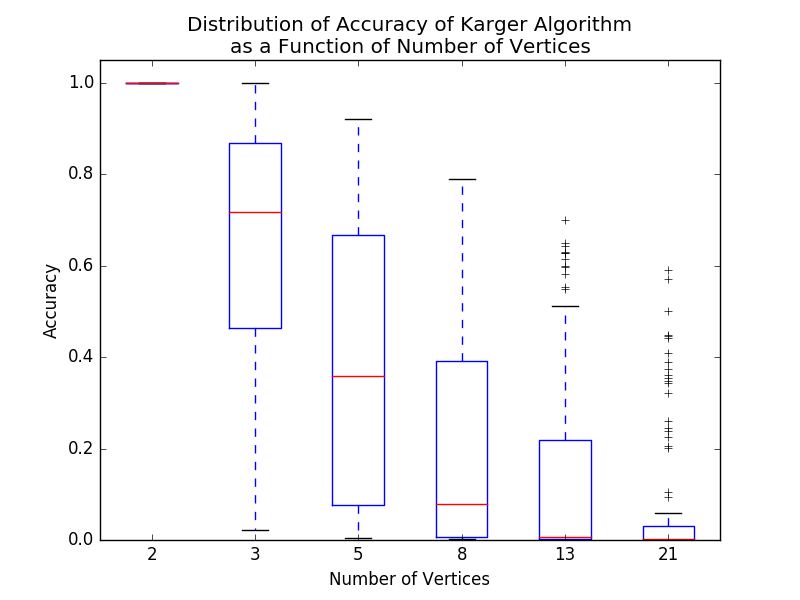
\includegraphics[scale=0.7]{karger.png}\\
\indent The above plot represents $10n^2$ runs of Karger's algorithm, on graphs of size n=[2,3,5,8,13,21].  As expected, accuracy on graphs of size 2 is 1.0, since there is only one edge to cut.  Karger's algorithm sees a 2-node graph as complete, and cuts any edges between the super nodes.  In the case of a 2-node graph, there is no edge collapsing or node merging to be done.  Just cut the one edge and return two nodes as the cut.  Accuracy decreases at an apparently logarithmic rate, quickly approaching zero as n increases, but levelling off as n grows.  Of interest is the high number of outliers in accuracy for n=21 graphs, while mean accuracy is very low.  While the 75th percentile appears to be well below 0.1 accuracy, there are several outliers in the 0.2 to 0.6 range.\\\\
4. b.  Let $G_n$ be a line graph of n nodes and (n-1) edges, such that (n-2) nodes have degree 2, and 2 nodes have degree 1.  When applied to G, Karger's will give an accuracy of 1.0.  In a graph such as this, every cut is a min-cut.\\
\indent Let $G'_n$ be a graph with an even number of nodes, n, where every node has degree 2.  The probability of Karger's algorithm finding a given min cut on a graph like $G'_n$ is given by $\frac{n-2}{n} * \frac{n-3}{n-1}*...*\frac{2}{3} = O(1/n^2)$.  Since there are n possible minimum cuts of weight 2, the probability of success of finding any one of these is $n(\frac{1}{n^2})=\frac{1}{n}$.\\
\indent Karger's algorithm will perform O(n) better on $G_n$ than on $G'_n$.\\\\\\\\
4. c.\\
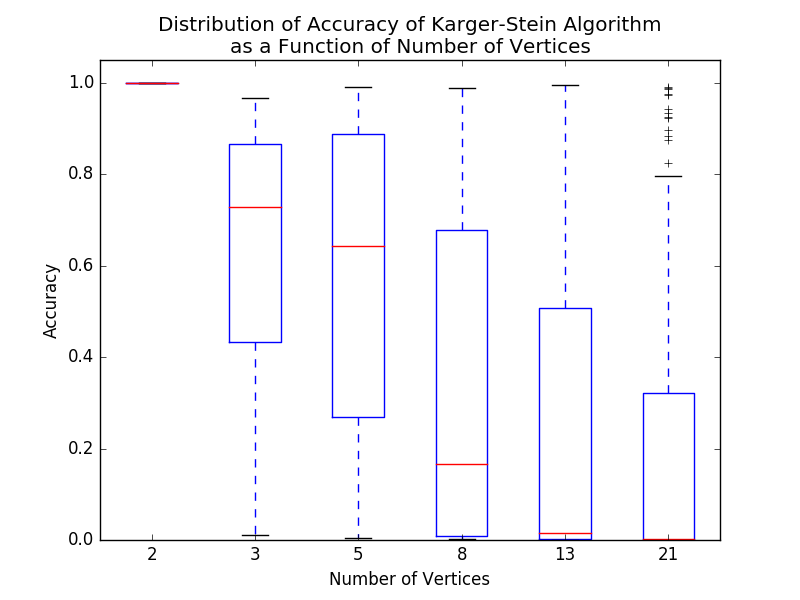
\includegraphics[scale=0.7]{kargerStein.png}\\
\indent The accuracy of the Karger-Stein algorithm is noticeably better than Kargers on all graph sizes, with the exception of n=2, where both show accuracy of 1.0.  The mean accuracy remains relatively high (above 0.6) until n grows larger than 5, when it quickly approaches 0.  However, even though mean accuracy is low for higher n values, the distribution is very wide, with the range given by 25th percentile to 75th percentile reaching up above 0.6 for n=8, and to approximately 0.3 for n=21.  The outliers for the n=21 graphs are extremely high, with some reaching very close to, if not achieving, an accuracy of 1.0.\\\\\\
5.  Given array P, consisting of all players, arranged in the same order as they are in the corridor:\\\\
\indent def chooseTeam(P,captain):\\
\indent\indent if len(P)==1:\\
\indent\indent\indent if captain ==A:\\
\indent\indent\indent\indent teamA.append(P[0])\\
\indent\indent\indent\indent return (P[0].score,teamA,teamB)\\
\indent\indent\indent if captain==B:\\
\indent\indent\indent\indent teamB.append(P[0])\\
\indent\indent\indent\indent return (-1*P[0].score,teamA,teamB)\\
\indent\indent else:\\
\indent\indent\indent if captain==A:\\
\indent\indent\indent\indent score1 = chooseTeam(P[1:],B)\\
\indent\indent\indent\indent score2 = chooseTeam(P[:-1]),B)\\
\indent\indent\indent\indent if score1 $>$ score2:\\
\indent\indent\indent\indent\indent score = score1 + P[0].score, teamA.append(P[0])\\
\indent\indent\indent\indent else:\\
\indent\indent\indent\indent\indent score = score2 +P[-1].score; teamA.append(P[-1])\\
\indent\indent\indent\indent  return (score, teamA,teamB)\\
\indent\indent\indent if captain==B:\\
\indent\indent\indent\indent score1 = chooseTeam(P[1:],B)\\
\indent\indent\indent\indent score2 = chooseTeam(P[:-1]),B)\\
\indent\indent\indent\indent if score1 $<$ score2:\\
\indent\indent\indent\indent\indent score = score1 - P[0].score, teamB.append(P[0])\\
\indent\indent\indent\indent else:\\
\indent\indent\indent\indent\indent score = score2 -P[-1].score; teamB.append(P[-1])\\
\indent\indent\indent\indent  return (score, teamA,teamB)\\


Call the function with chooseTeam(P,A), since A gets first choice.  A's team will consist of choices that maximize $score$, while B's team will consist of players that minimize $score$.\\\\
Correctness: In this algorithm, the choices for captain A are those that maximize the score, while captain B will be attempting to minimize it.  A good choice for A is bad for B, and vice versa.  At each level, B will choose the results from the recursive call that gives a lower score, while A will choose the results from the recursive call that results in the highest score.  In this manner, each captain will maximize the ability of her team.\\
Runtime:  The recursive function will be called $n^2$ times, where n is the number of players.  Each call will result in two more calls, examining the results of choosing the first or last player in line.  The recursion halts when there is only one player remaining to be chosen. Runtime is $O(n^2)$\\\\\\
6.  If the array is already sorted (best case), then insertion sort runs in O(n) time, since the inner loop is never triggered.  Insertion sort simply compares each A[j] and A[j-1] and moves on to the next index j+1.  Each time the inner loop is triggered (k times in a k-nearly sorted array), the additional runtime is O(n), as the elements are swapped, moving through the array as j = j - 1, until A[j-1] $\leq$ A[j].  This results in O(n) + O(kn) , or O(kn), runtime.\\\\\\\\
7. def flipTiles(n)\\
\indent\indent j = ceiling(log(n)/log(4))\\
\indent\indent for i in range(0, j-1):\\
\indent\indent\indent OP2() \#op2 on all face up tiles\\
\indent\indent while ($|FU|>0$):\\
\indent\indent\indent OP1() \#flip manually\\\\
Correctness:  The cost of performing OP1 at any given time is equal to the number of face-up tiles, $|FU|$.  The cost of OP2 is given by $\frac{n}{number\ tiles\ flipped}$.  Since it is wasteful to include face-down tiles in OP2, and we want to maximize the number of tiles flipped for every OP2 performed, as well as minimize the cost by making the denominator as large as possible, the cost of OP2 is $\frac{n}{|FU|}$.  Since the probability for any face up tile becoming face down in OP2 is 0.5, the cost of i iterations of OP2 is $\frac{n}{n} + \frac{n}{\frac{n}{2}} +\frac{n}{\frac{n}{4}} +... + \frac{n}{\frac{n}{2^{i-1}}}=1+2+4+...+2^{i-1} =2^i-1$.  As OP2 is not guaranteed to ever return 0 face up tiles, the minimum cost to turn all tiles face down after i iterations is $2^i -1$ + (some positive value C), or at least $2^i$.\\
\indent When the cost to finish the job using OP1 is less than or equal to the cost of finishing with OP2, stop use of OP2.  The value j in $flipTiles(n)$ is simply a measure of this point.  Cost of finishing with OP2 is at least $2^i$ and cost of finishing with OP1 is $|FU|$(cost of OP1 after i iterations of OP2 is $\frac{n}{2^i}$).  The decision point is given by the inequality $\frac{n}{2^i} \leq 2^{i-1}$.  Solving for i gives $i\geq \frac{log\ n}{log\ 4}$\\\\
Runtime:  We stop using OP2 after i = ceiling($\frac{log\ n}{log\ 4}$) rounds because the cost of finishing with OP1 is less that (i+1) rounds of OP2.  This is the worst-case boundary.  The cost of (i+1) rounds of OP2 is $2^{\frac{log\ n}{log\ 4}+1}$.  This gives $O(n^{\frac{1}{2}}).$\\
\\
8.  def rightSpot(numberOpenSpots):\\
\indent\indent if numberOpenSpots==1:\\
\indent\indent\indent return 1\\
\indent\indent else:\\
\indent\indent\indent return = rightSpot(numberOpenSpots-1) * $\frac{1}{numberOpenSpots}$\\\\
\indent Correctness:  The probability that a given minion stands in the correct spot (given the correct spot is not occupied) is $\frac{1}{number\ of\ unoccupied\ spots}$  The probability that the minion's assigned spot is unoccupied is a function of all minions before him (her?).  For the last minion, Pr(minion$_n$ stands in correct spot $|$ all previous minions stand in correct spot) = 1 * Pr(Minion$_{n-1}$ in correct spot $|$ minions$_{n-2}$...minion$_1$ stand in correct spot).  Total probability that all minions are in the correct spot is $\prod_{i=1}^n(\frac{1}{i}) = \frac{1}{n!}$\\

%Given: $p=\frac{k}{2^n}$ where n = number of calls to randbit() by randbit(p)\\\\
%\indent Since randbit() returns 0 or 1, the number of possible results after n calls to randbit() is $2^n$.\\
%\indent $p=\frac{k}{2^n}$, so of the $2^n$ possible results from n calls to randbit(), k of these results 


\end{document} 
